\newpage
\section{TCGAbiolinksGUI: A graphical user interface to analyze GDC cancer molecular and clinical data}

Although TCGAbiolinks is a suitable R package for most data analysts with a strong knowledge and familiarity with R specifically those who can comfortably write R commands, we developed TCGAbiolinksGUI to enable user access to the methodologies offered in TCGAbiolinks and to give users the flexibility of point-and-click style analysis without the need to enter specific arguments. TCGAbiolinksGUI takes in all the important features of TCGAbiolinks and offers a graphics user interface (GUI) thereby eliminating any need to familiarize TCGAbiolinks' key functions and arguments.

\subsection{Infrastructure}
The TCGAbiolinksGUI user interface was created using Shiny, a Web Application Framework for R, and uses several packages to provide advanced features that can enhance Shiny apps, such as shinyjs to add JavaScript actions \cite{shinyjs}, shinydashboard to add dashboards \cite{shinydashboard} and shinyFiles \cite{shinyFiles} to provide access to the server file system.

The following R/Bioconductor packages are used as back-ends for the data retrieval and analysis: TCGAbiolinks \cite{TCGAbiolinks} which allows to search, download and prepare data from the NCI's Genomic Data Commons (GDC) data portal into an R object and perform several downstream analysis;  ELMER (Enhancer Linking by Methylation/Expression Relationship) \cite{yao2015inferring, ELMER2} which identifies DNA methylation changes in distal regulatory regions and correlate these signatures with the expression of nearby genes to identify transcriptional targets associated with cancer; ComplexHeatmap \cite{Gu20052016} to visualize data as oncoprint and heatmaps, pathview \cite{luo2013pathview} which offers pathway based data integration and visualization; and maftools \cite{Maftools} to analyze, visualize and summarize \sigla{MAF}{Mutation Annotation Format} files.


\subsection{Graphical user interface design}
The user interface has been divided into three main \sigla{GUI}{Graphical User Interface} menus. The first menu defines the acquisition of GDC data. The second defines the analysis steps which subdivides according to the molecular data types.  And the third is dedicated to harnessing integrative analyses. We present below a brief description of each menu and their features that can be accessed through a side panel (see figure \ref{fig:fig1}):

\begin{figure}
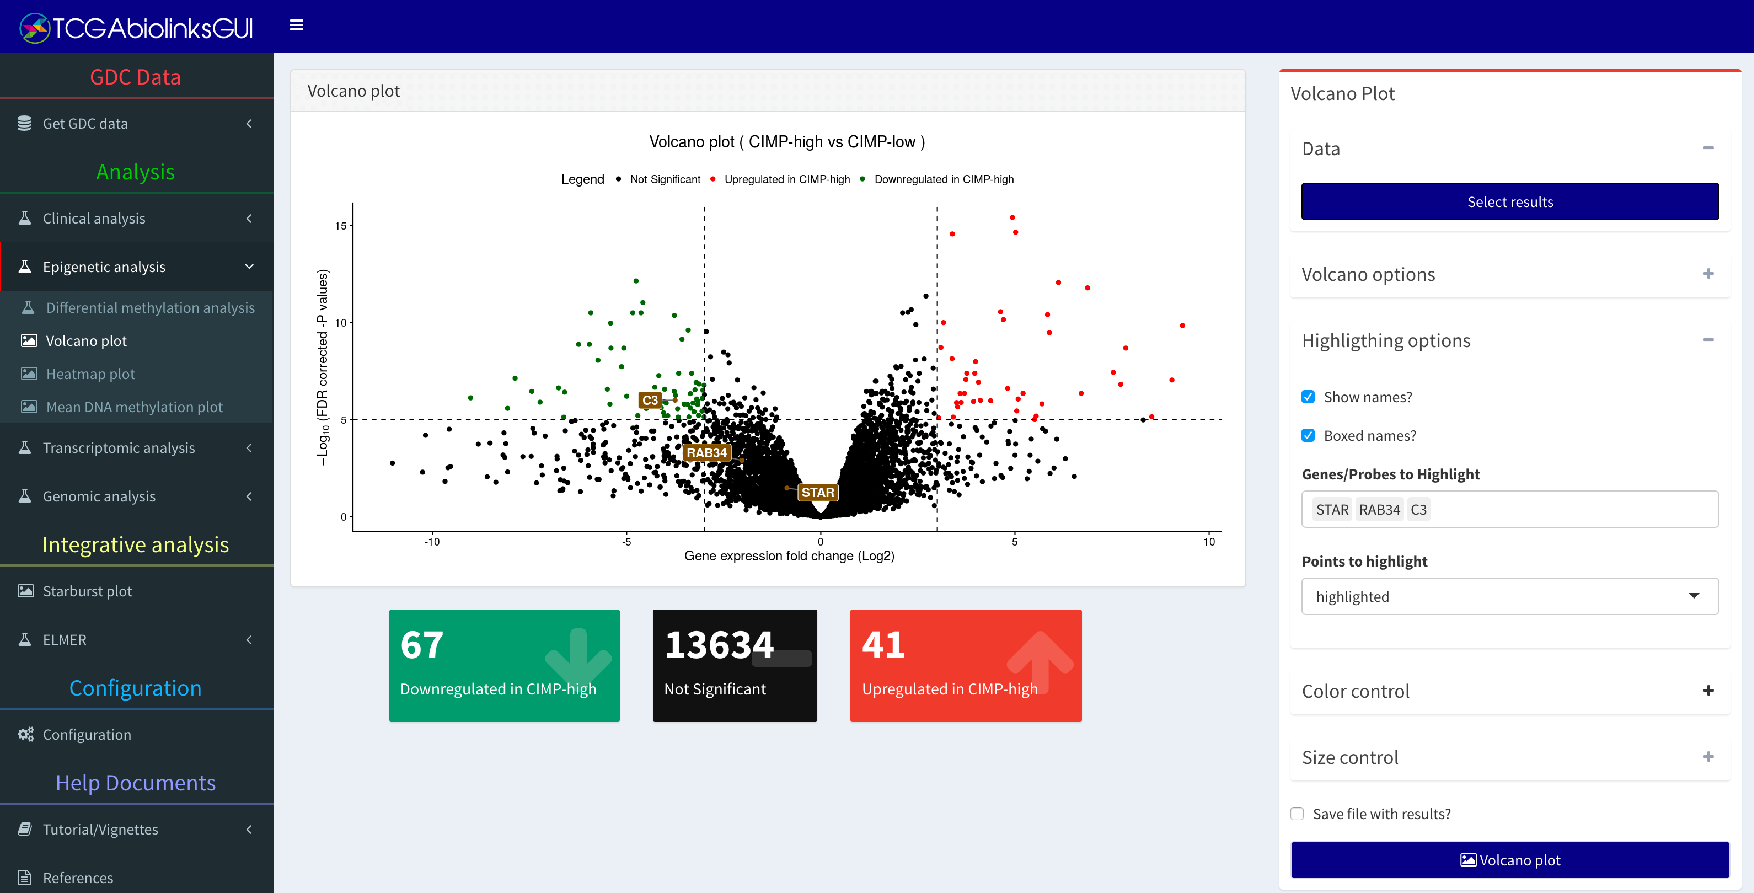
\includegraphics[width=1.0\linewidth]{images/fig1-GUI.pdf}
\caption[TCGAbiolinksGUI: The volcano plot menu]{The volcano plot menu of TCGAbiolinksGUI: The panel on the left shows the menus divided by different analyses, the panel on the right shows the controls available for the menu selected. In the center is a volcano plot window from the  analysis menu. It is possible to control the colors, to change cut-offs and to export results into a CSV document.}
\label{fig:fig1}
\end{figure}

\begin{figure}
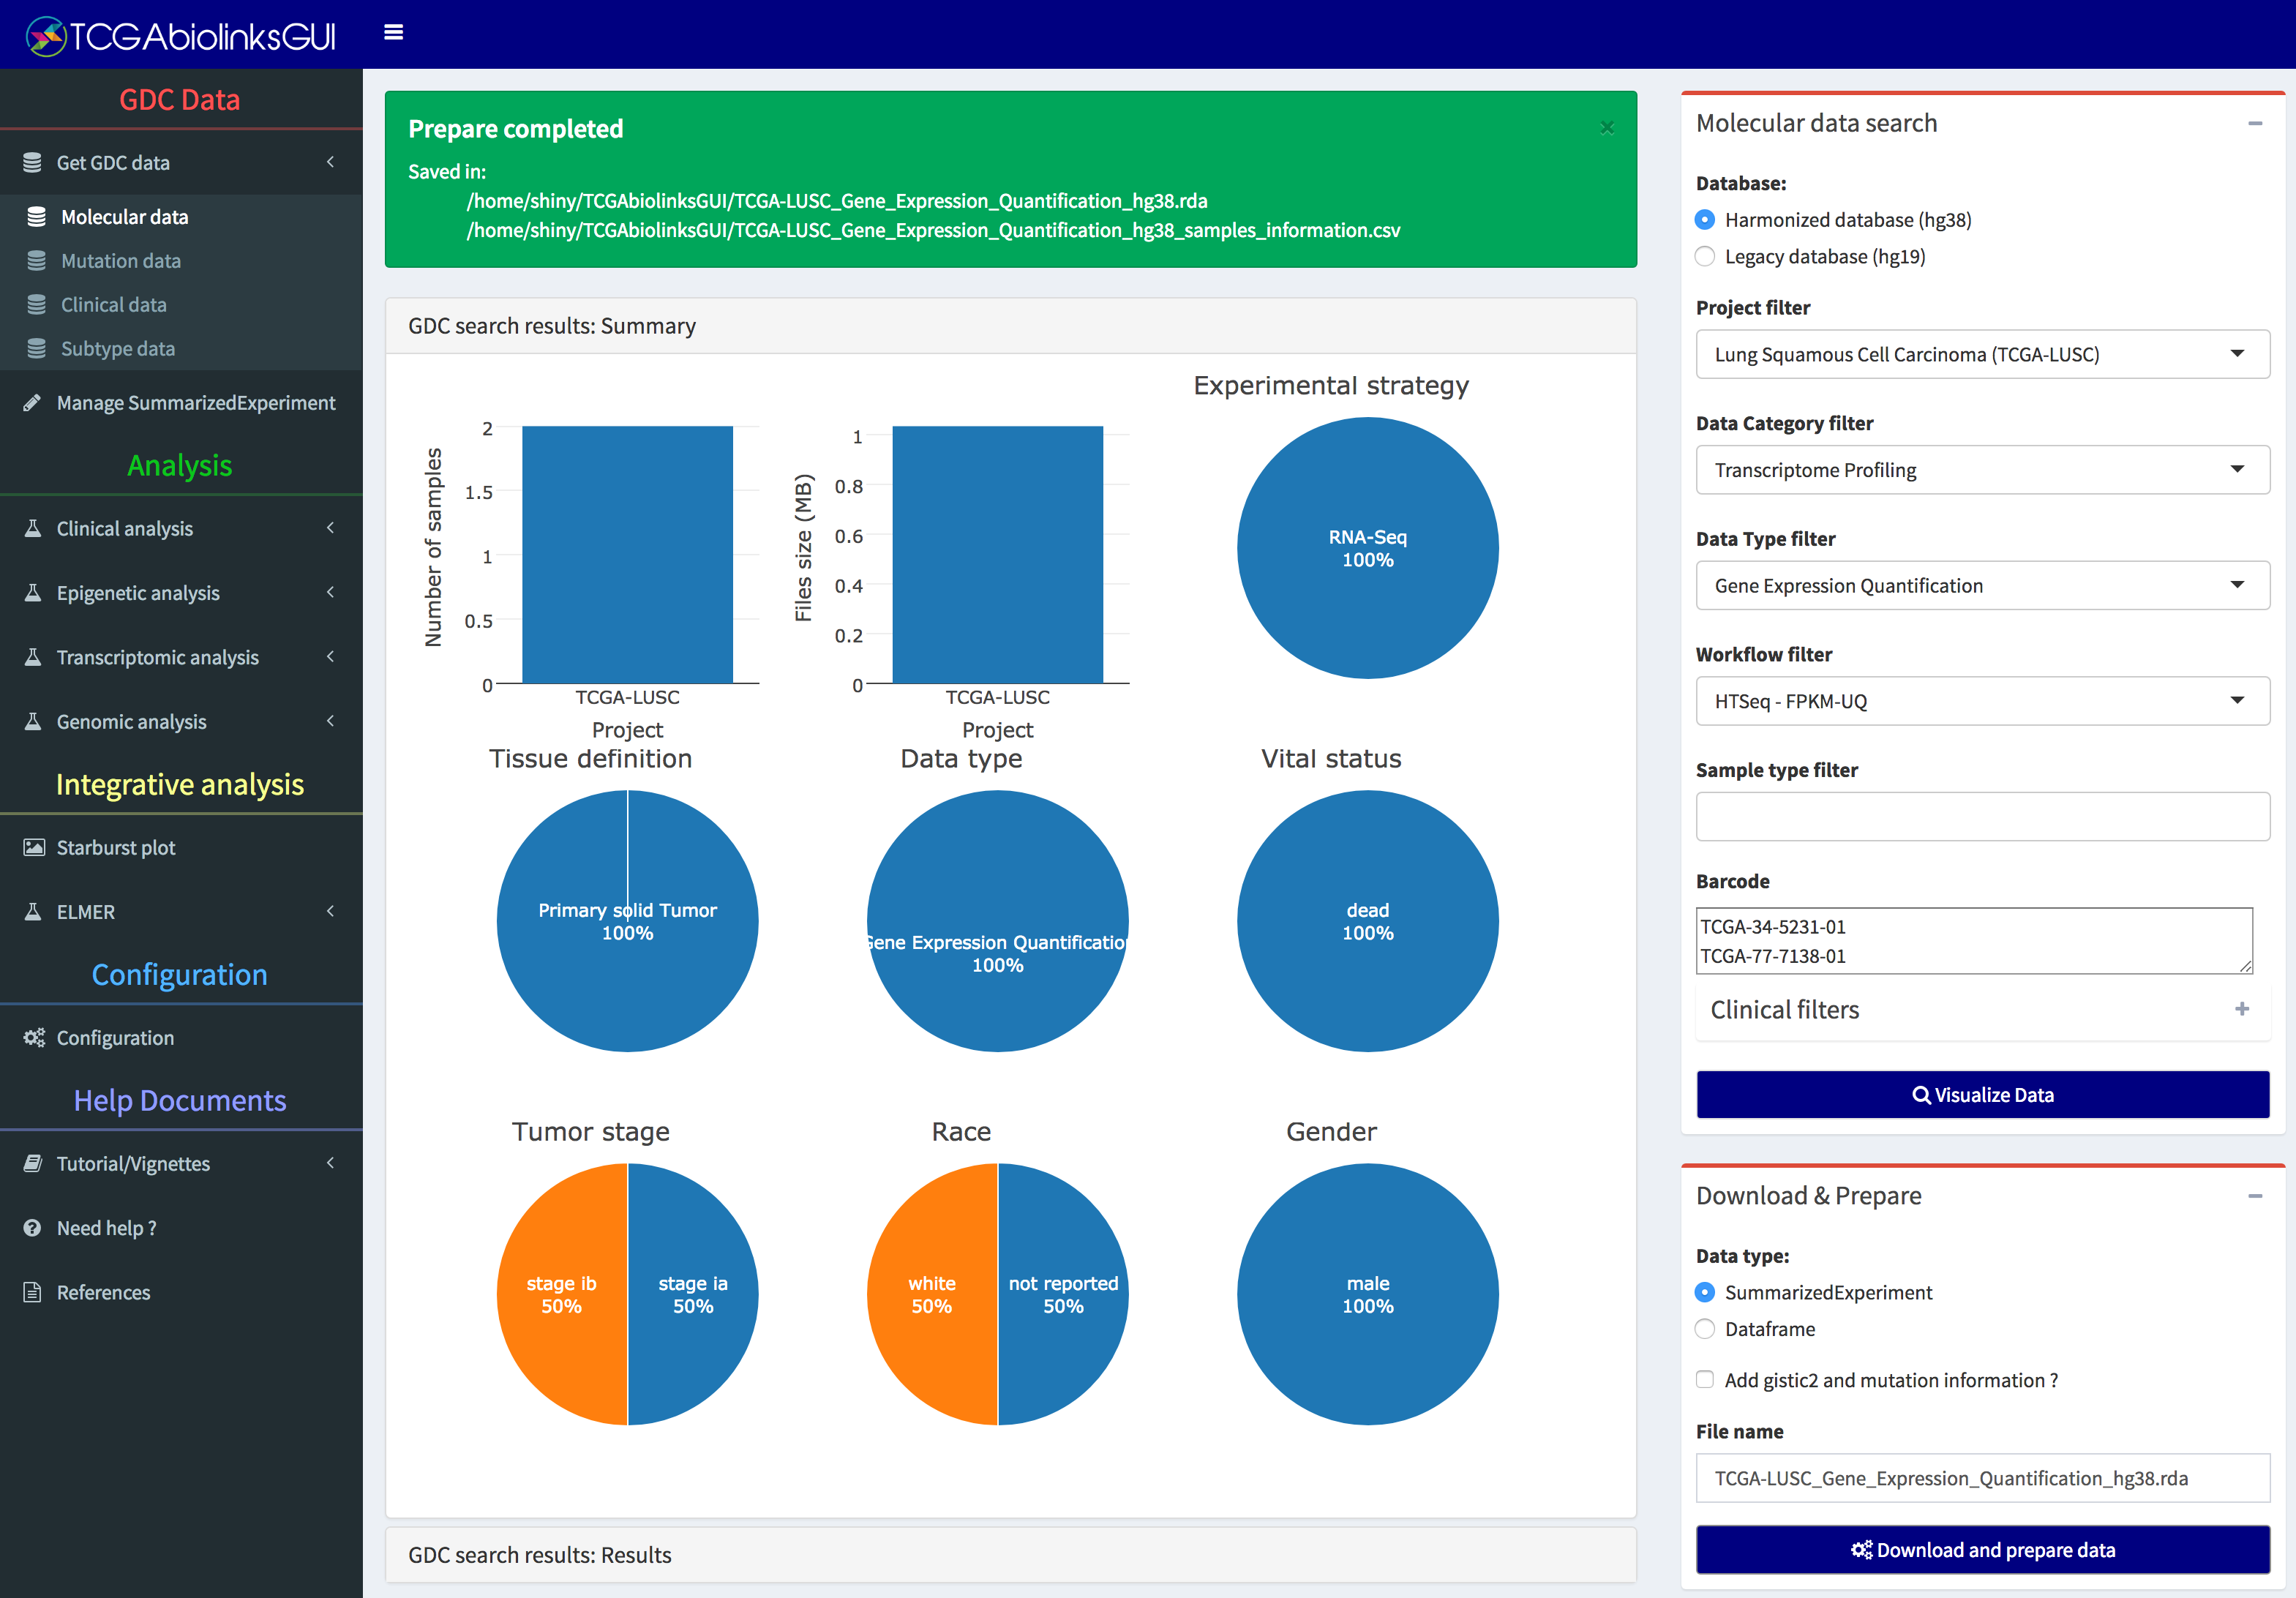
\includegraphics[width=1.0\linewidth]{images/fig2-Data_expression.png}
\caption[TCGAbiolinksGUI: Gene expression download: ]{Molecular data download: Gene expression Search, download and prepare into an R object of gene expression data for two TCGA-LUSC samples ("TCGA-34-5231-01","TCGA-77-7138-01"). The Summarized Experiment object created is saved as an RData file (TCGA-LUSC-Gene\_Expression\_Quantification\_hg38.rda). }
\label{fig:geneexp}
\end{figure}

\begin{itemize}
\item \textbf{GDC Data:} Provides a guided approach to search for published molecular subtype information, clinical and molecular data. In addition, it downloads and processes the molecular data into an R object that can be used for further analysis (Figure \ref{fig:geneexp})
\item \textbf{Clinical analysis:} Performs survival analysis to quantify and test survival differences between two or more groups of patients and draws survival curves with the 'number at risk' table, the cumulative number of events table and the cumulative number of censored subjects table using the R/CRAN package survminer \cite{survminer} (Figure \ref{fig:gui_survival}).
\item \textbf{Epigenetic analysis:} Performs a Differentially methylated regions (DMR) analysis, visualizes the results through both volcano and heatmap plots, and visualizes the mean DNA methylation level by groups (Figure \ref{fig:gui_heatmap}).
\item \textbf{Transcriptomic analysis:} Performs a Differential Expression Analysis (DEA), and visualizes the results through both volcano and heatmap plots. For the genes found as upregulated or downregulated an enrichment analysis can be performed and pathway data can be integrated \cite{luo2013pathview}.
\item \textbf{Genomic analysis:} Visualize and summarize the mutations from MAF (Mutation Annotation Format) files through summary plots and oncoplots using the R/Bioconductor maftools package \cite{Gu20052016,Maftools}
(Figures \ref{fig:maftoools_oncoplot} and \ref{fig:maftoools_summary}).
\item \textbf{Integrative analysis:} Integrate the DMR and DEA results through a starburst plot. Also, using the DNA methylation data and the gene expression data the R/Bioconductor ELMER package can be used to discover functionally relevant genomic regions associated with cancer \cite{yao2015inferring, ELMER2}.
\end{itemize}


\begin{figure}
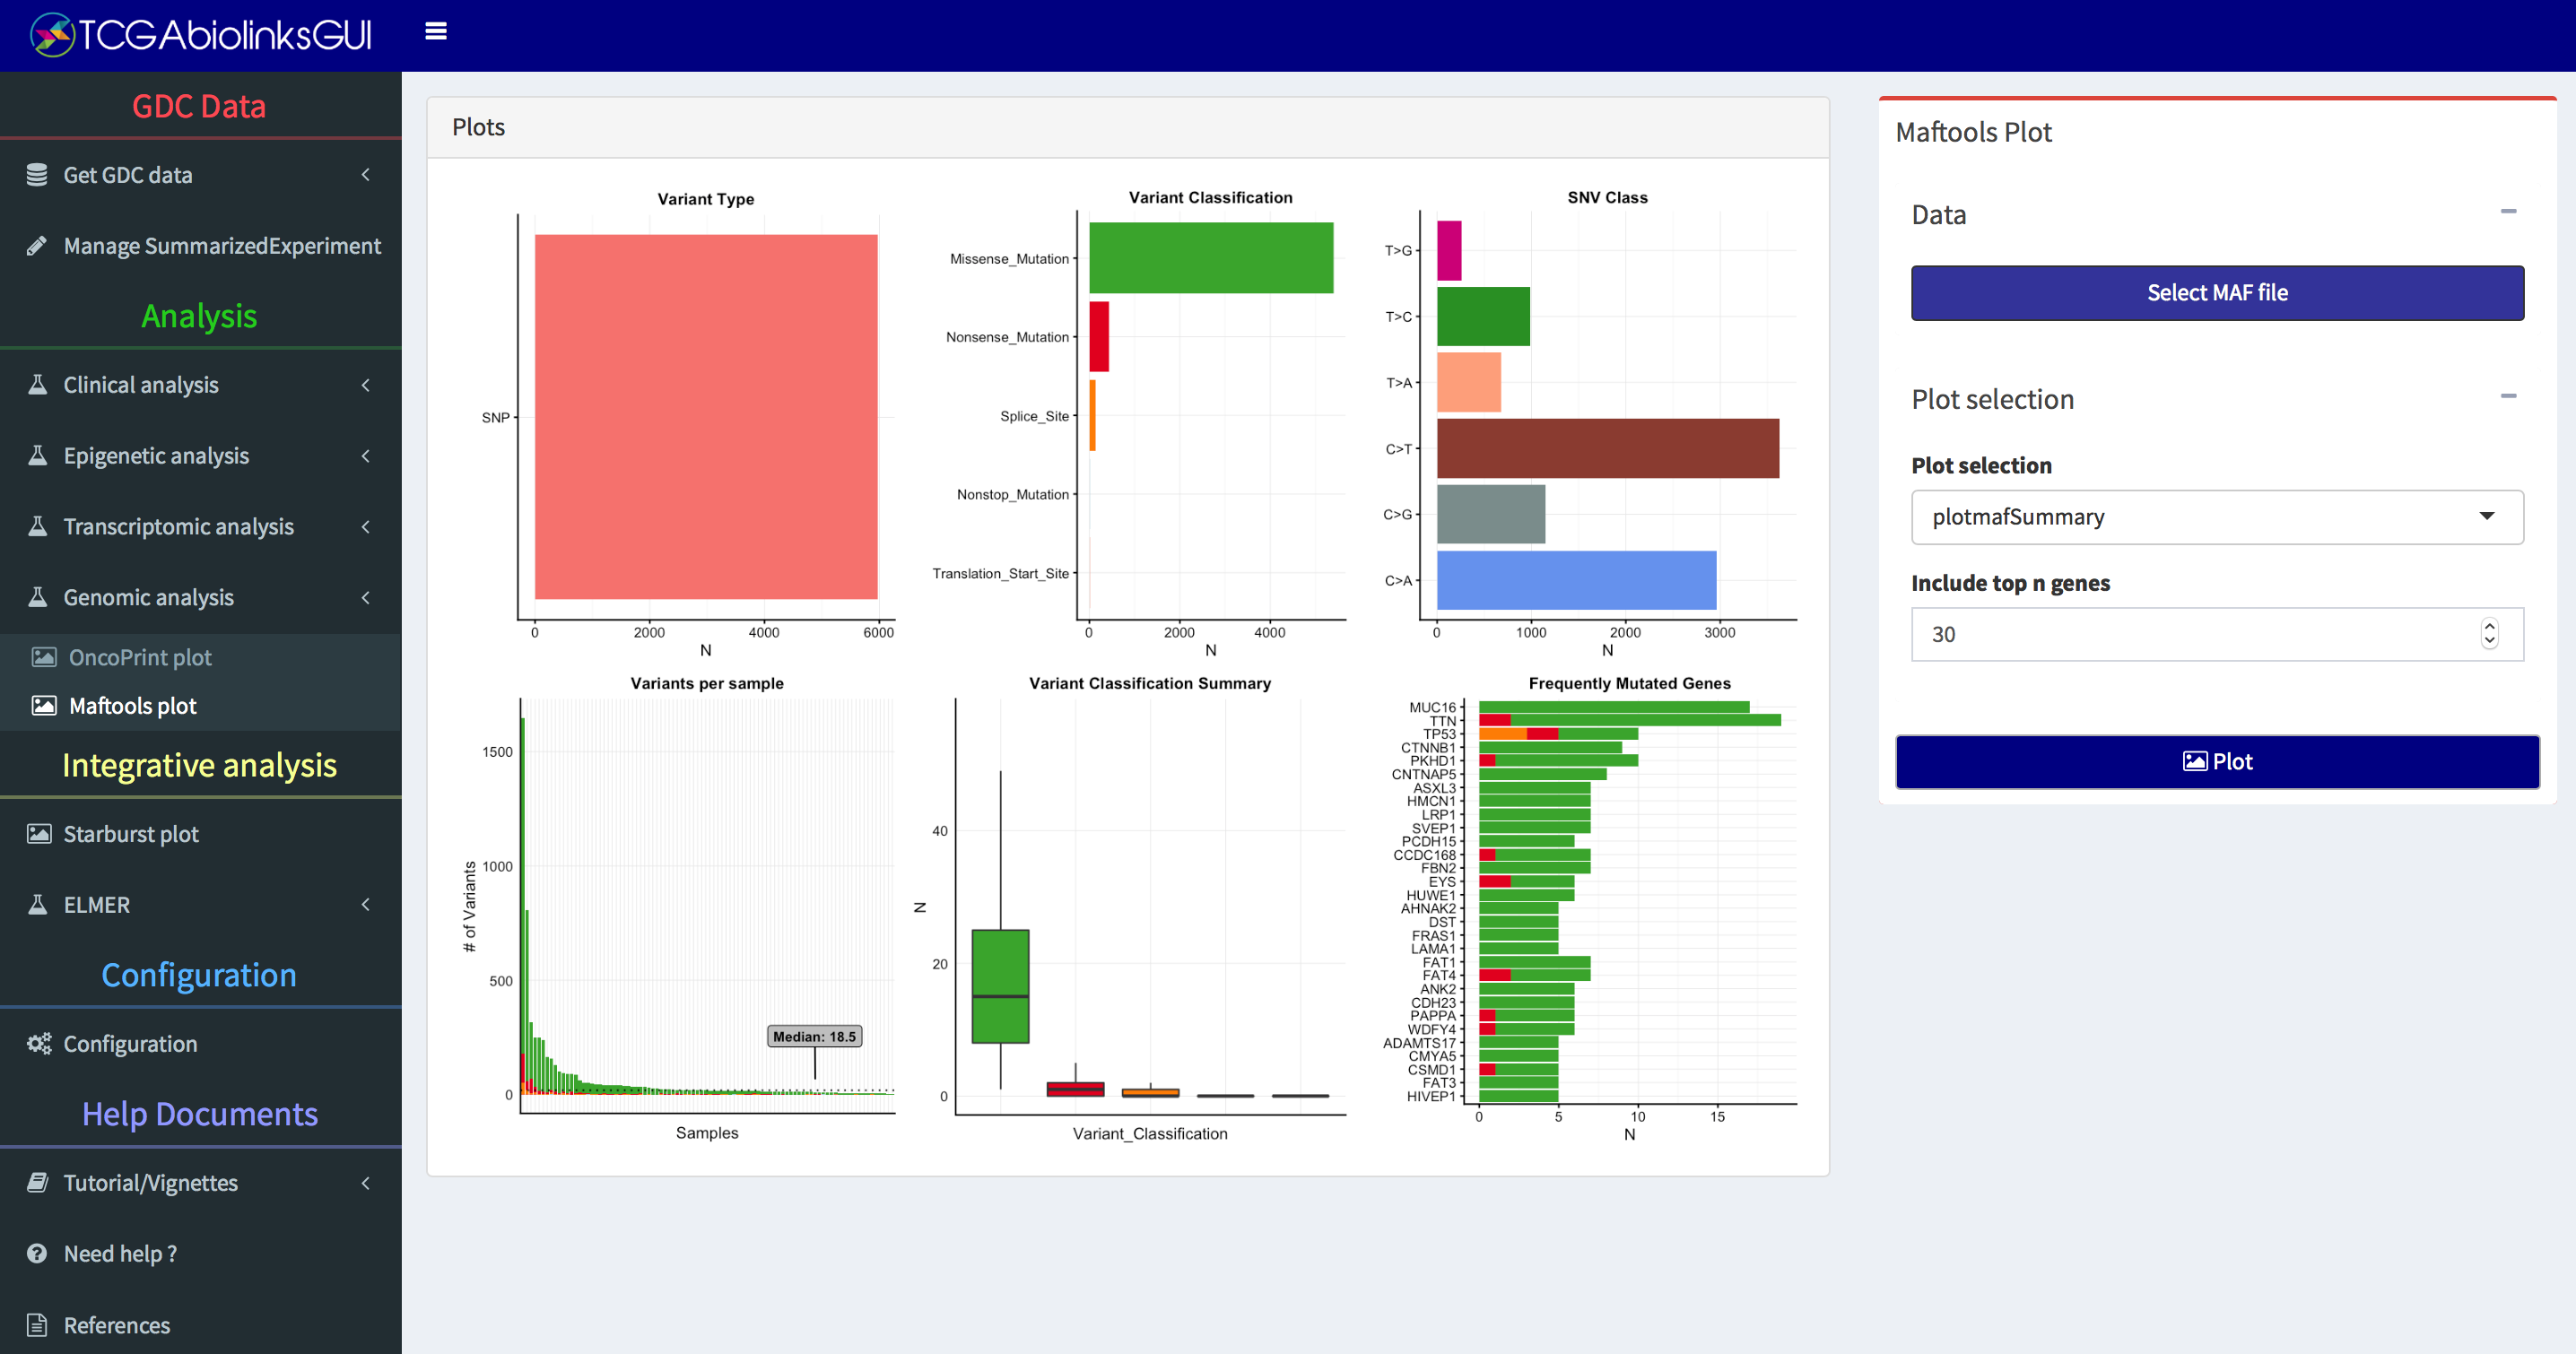
\includegraphics[width=1.0\linewidth]{images/maftools_summary.png}
\caption[TCGAbiolinksGUI: Visualizing mutation summary]{TCGAbiolinksGUI: Visualizing mutation summary. This maftools plot available thought TCGAbiolinksGUI shows a summary of the MAF file. Highlighting the most mutated genes, SNV class and variant classification distributions. }
\label{fig:maftoools_summary}
\end{figure}

\begin{figure}
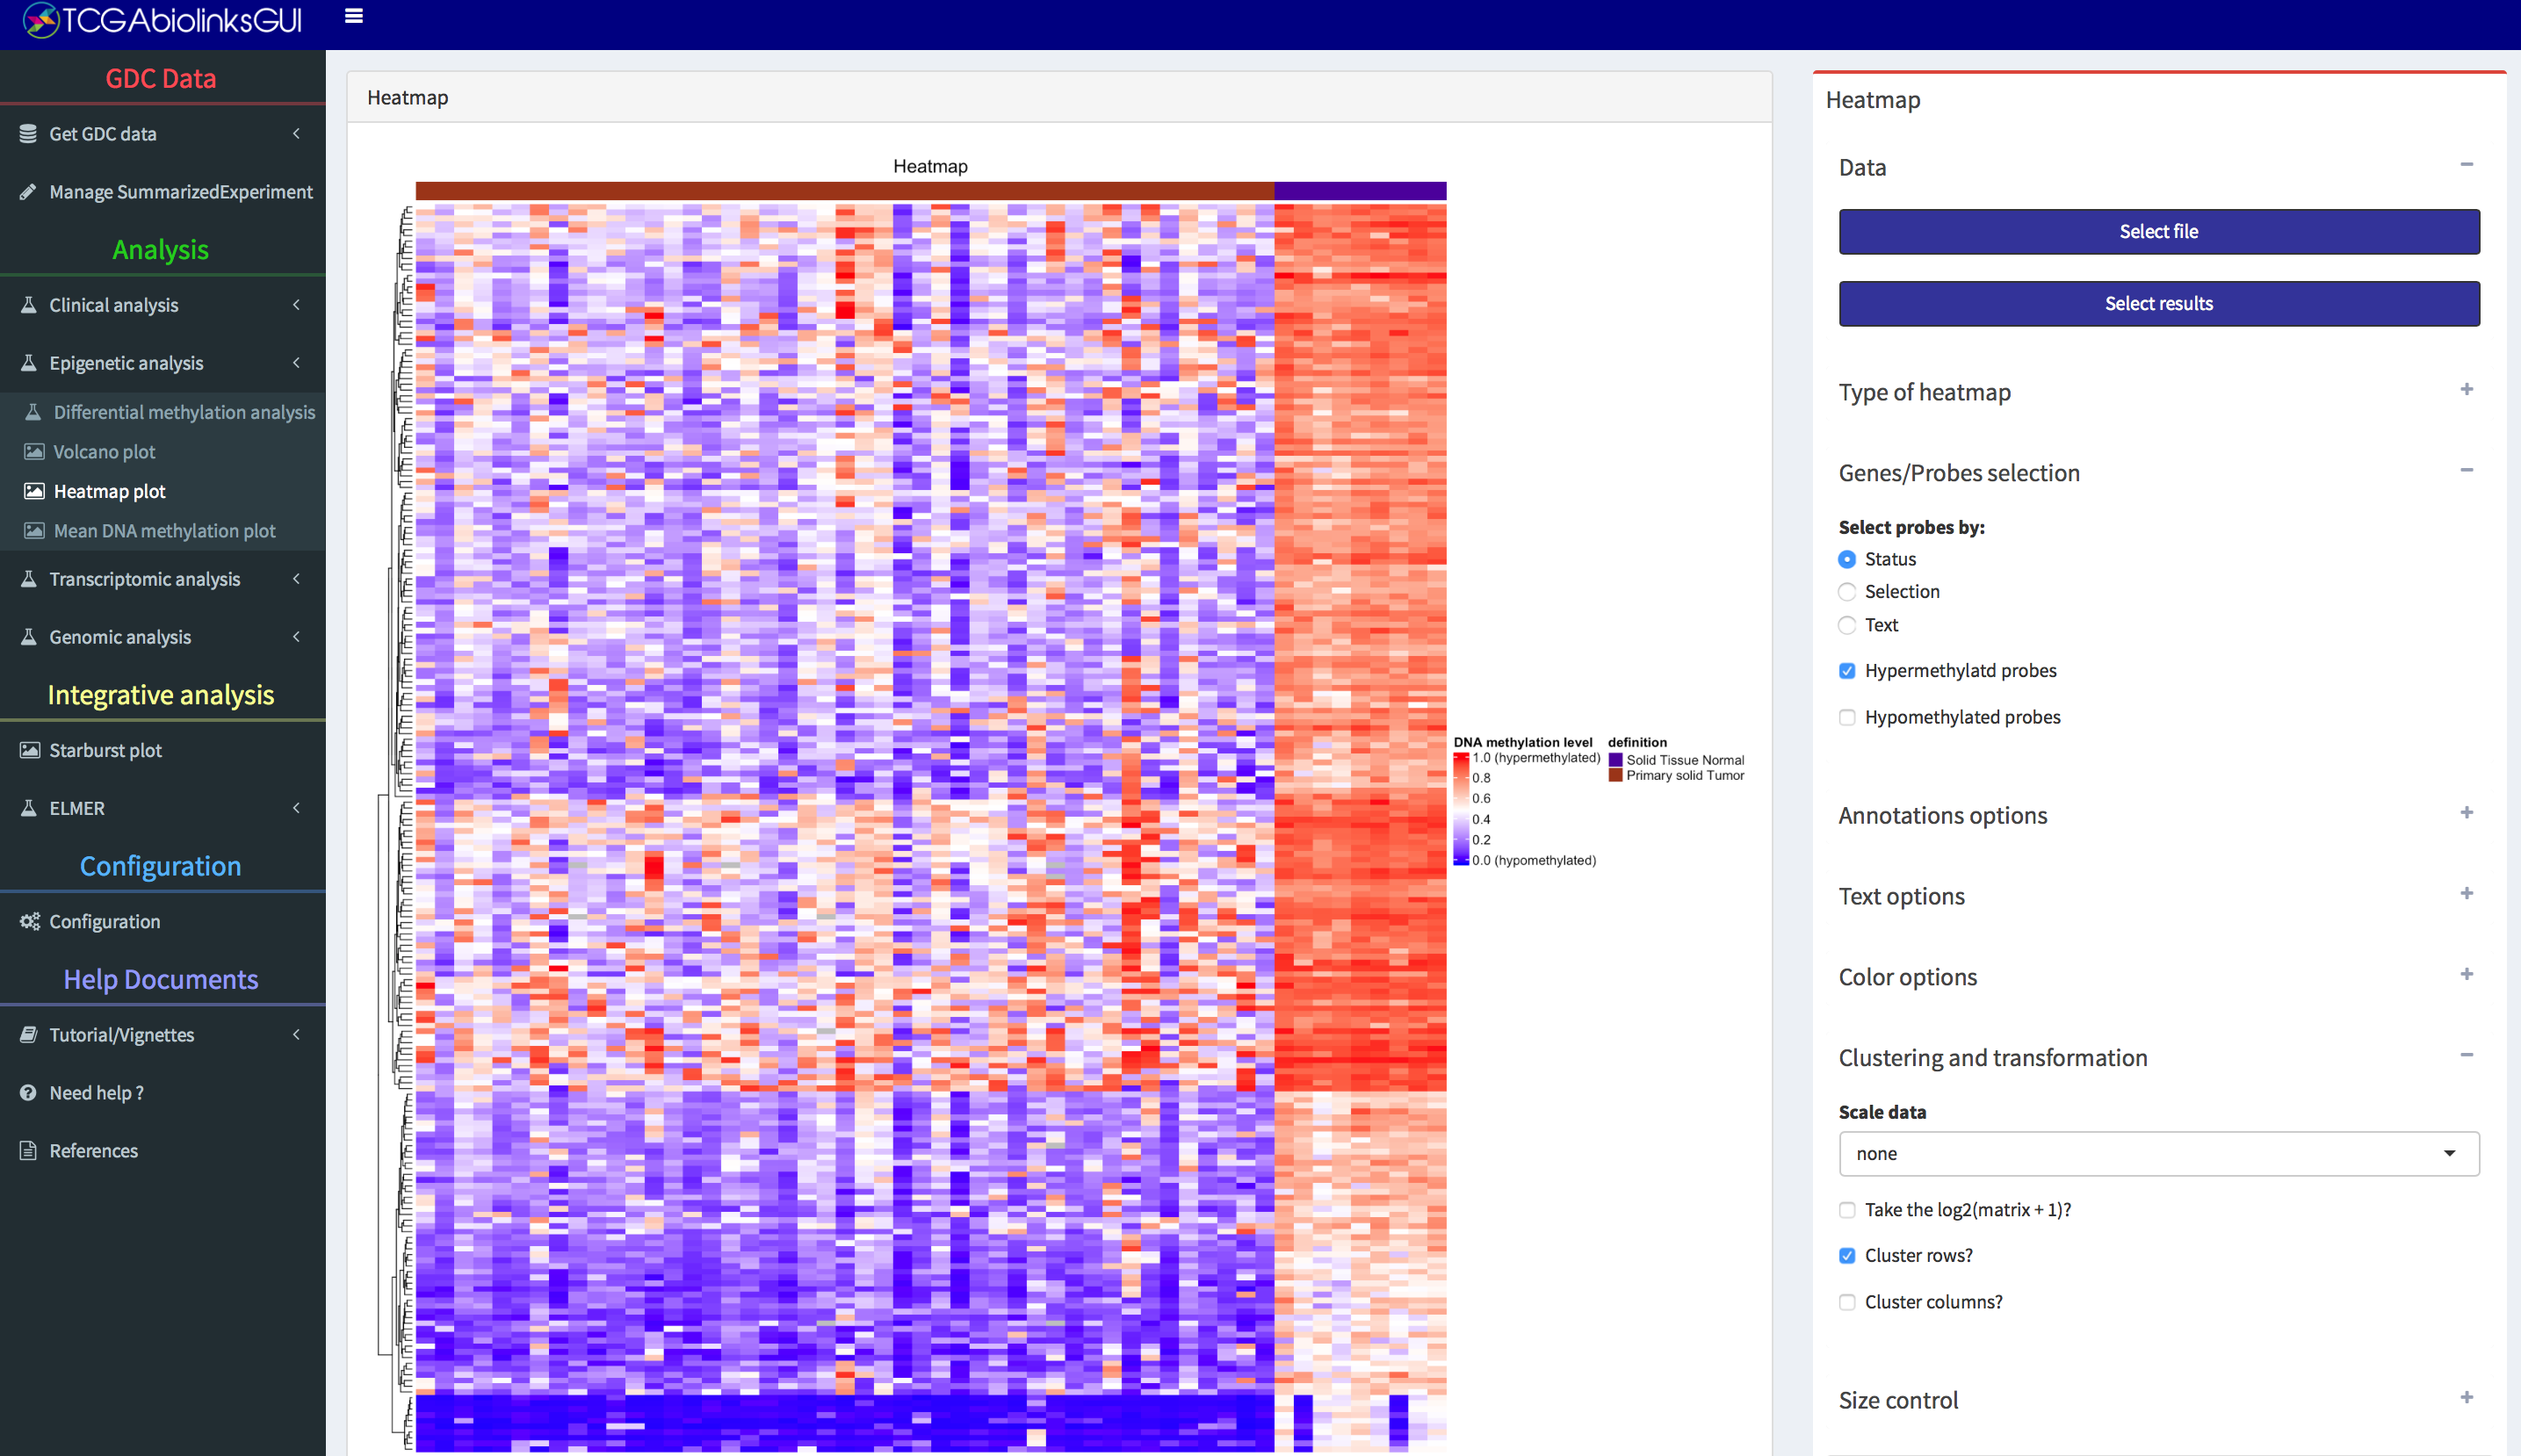
\includegraphics[width=1.0\linewidth]{images/gui_heatmap.png}
\caption[TCGAbiolinksGUI: Visualizing DMR results as heatmap]{TCGAbiolinksGUI: Visualizing DMR results as heatmap. Plot shows the DMR results: hypermethylated probes in Solid tissue normal samples compared to the Primary Solid tumor samples. Each column is a sample, while each row is a probe. Blue colors represents probes with low levels of DNA methylation and red the ones with high level. }
\label{fig:gui_heatmap}
\end{figure}


\begin{figure}
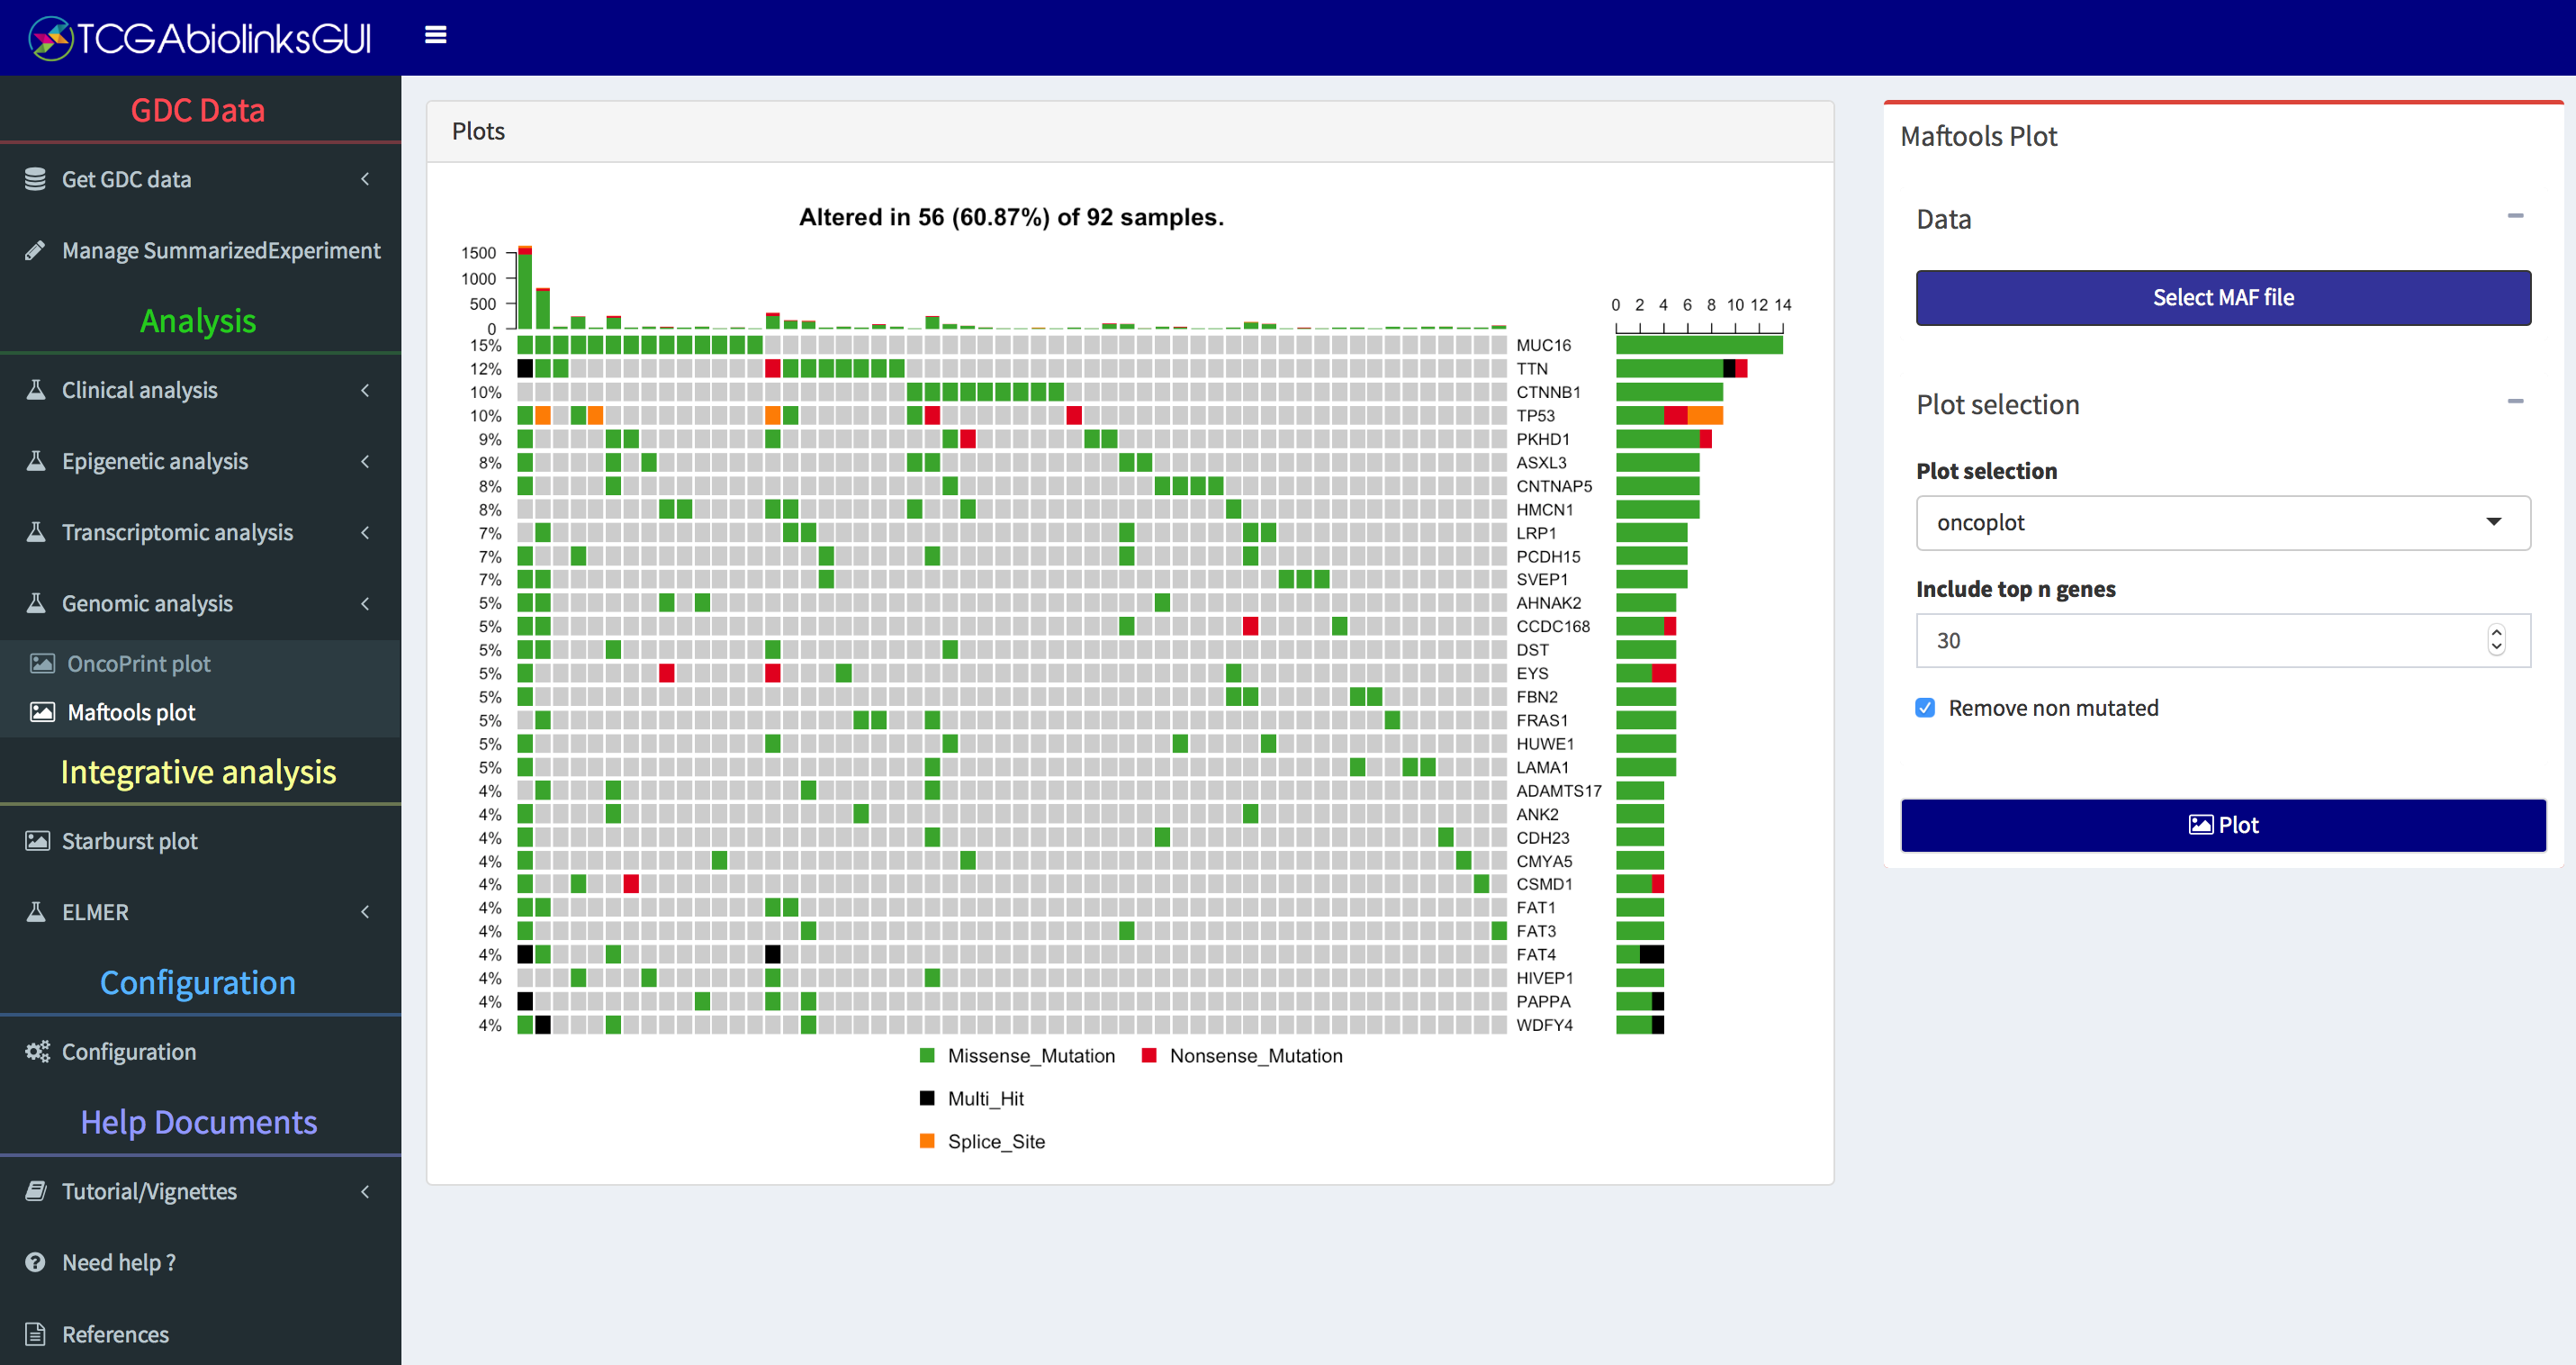
\includegraphics[width=1.0\linewidth]{images/maftools_oncoplot.png}
\caption[TCGAbiolinksGUI: Visualizing mutation as an oncoplot]{TCGAbiolinksGUI:Visualizing mutation as an oncoplot. Each column
represents a sample and each row a different gene. The top barplot has the frequency of mutations for each patient, while
the right barplot has the frequency of mutations for each gene. The plot by deafult is ordered by the most mutated genes.}
\label{fig:maftoools_oncoplot}
\end{figure}


\begin{figure}[]
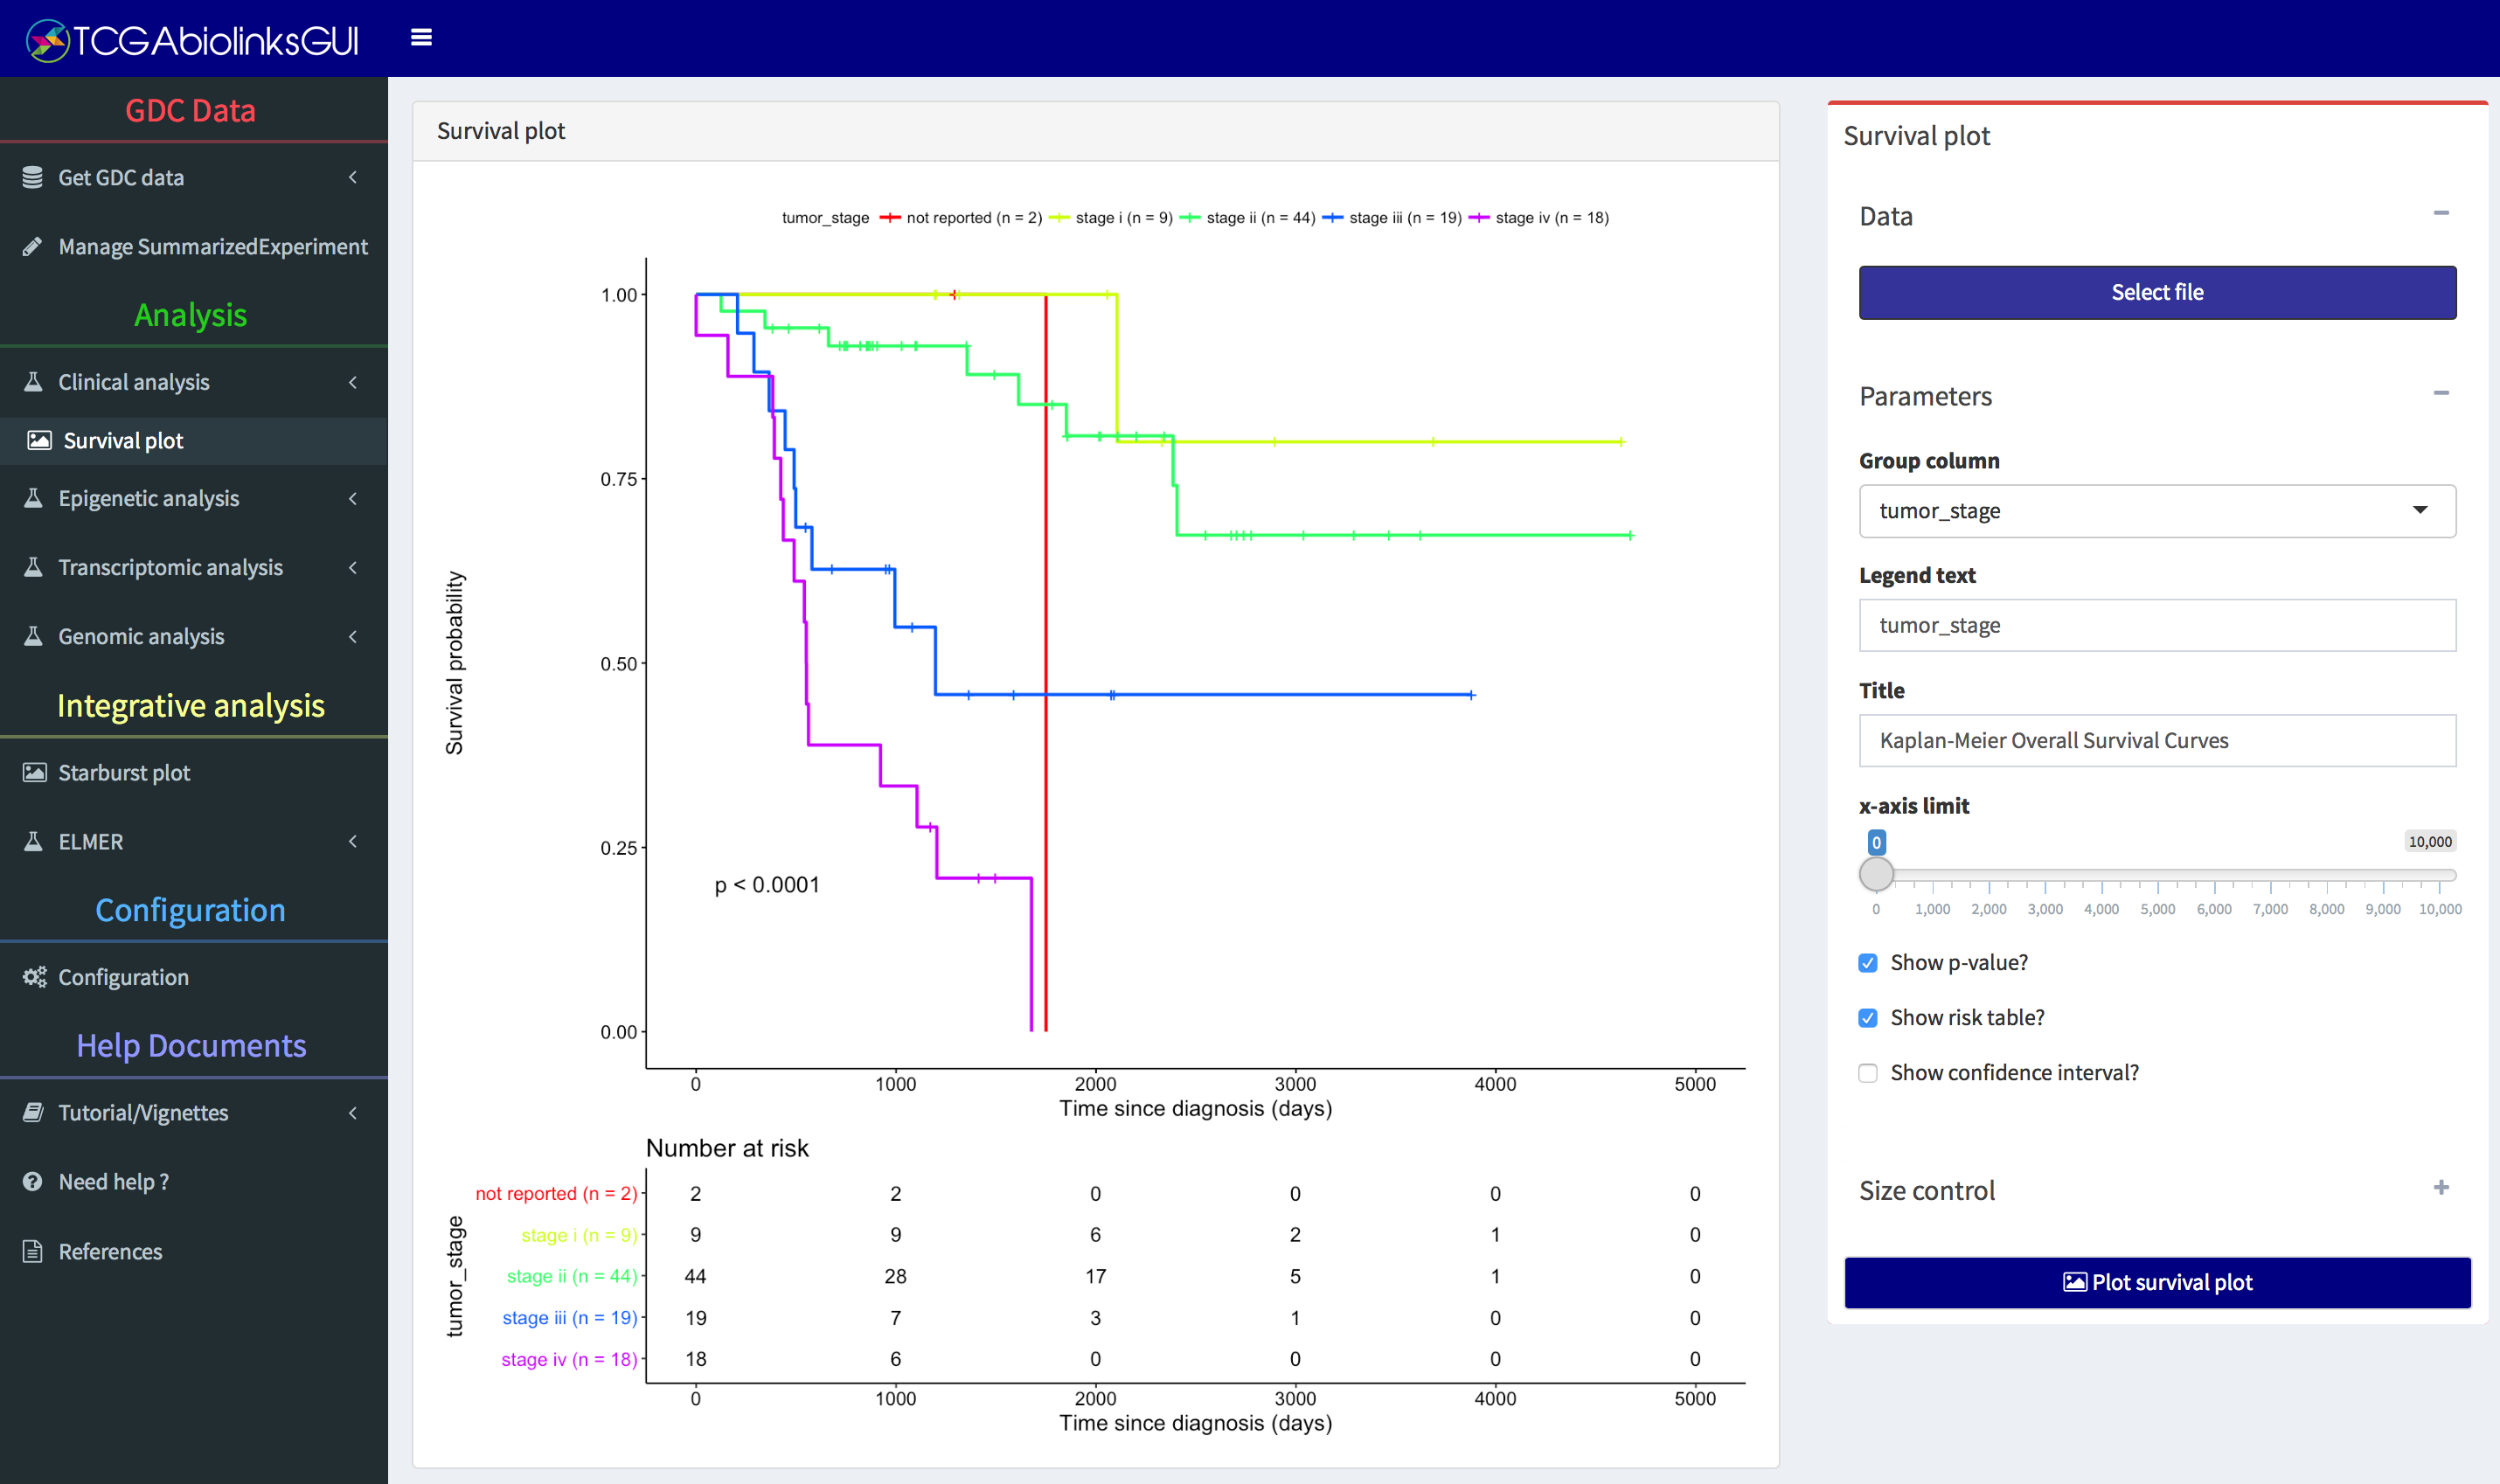
\includegraphics[width=1.0\linewidth]{images/gui_acc_survival.png}
\caption[TCGAbiolinksGUI: Survival analysis]{TCGAbiolinksGUI: Survival analysis.
The plot shows the Kaplan-Meier Overall Survival Curves for ACC (Adrenocortical carcinoma) stratified by tumor stage.
As expected, hihger levels which are more agressive have a lower survival.}
\label{fig:gui_survival}
\end{figure}

\subsection{Documentation}

We provide a guided tutorial for users via a vignette document which details each step and menu function available at \href{http://bit.do/TCGAbiolinksDocs}{http://bit.do/TCGAbiolinksDocs}, via online documents available at
\href{http://bit.ly/TCGAbiolinks\_PDFTutorials}{http://bit.ly/TCGAbiolinks\_PDFTutorials}, and via YouTube video instructions showing step by step how each menu works available at \href{http://bit.ly/TCGAbiolinksGUI\_videoTutorials}{http://bit.ly/TCGAbiolinksGUI\_videoTutorials}, which assist end-users in taking full advantage of TCGAbiolinksGUI. A demonstration version of the tool is available at \href{http://tcgabiolinks.fmrp.usp.br:3838/}{http://tcgabiolinks.fmrp.usp.br:3838/}. Users are encouraged to report and file bug reports or feature requests via our GitHub repository \href{https://github.com/BioinformaticsFMRP/TCGAbiolinksGUI/issues}{BioinformaticsFMRP/TCGAbiolinksGUI/issues}.

\subsection{Docker container}
To further simplify the usability and accessibility of our tool, we provide a docker image compatible with most popular operating system available at \\
\href{https://hub.docker.com/r/tiagochst/tcgabiolinksgui/}{https://hub.docker.com/r/tiagochst/tcgabiolinksgui/}. This file allows users to run TCGAbiolinksGUI without the need to install associated dependencies or configure system files, common steps required to run R installations and load R/Bioconductor packages.

\subsection{Comparison of alternative software}

Web tools used for cancer data analysis might be classified into two broad groups.
The first group only provides an interface to existing software analysis tools.
The Galaxy project (\href{https://galaxyproject.org/}{https://galaxyproject.org/}), which is an open, web-based platform for accessible, reproducible, and transparent computational biomedical research, is an example of such a tool that belongs to this group.
The other group is composed of exploratory tools mainly focused on the visualization of processed data and pre-computed results. The cBioPortal project \cite{gao2013integrative,cerami2012cbio}, by providing several visualizations for mining the TCGA data, is an example of a tool that falls within this classification.

If one were to classify TCGAbiolinksGUI, it would belong to the first group. Compared to the Galaxy project, TCGAbiolinksGUI offers an open platform which improves the accessibility of R/Bioconductor packages, allowing users an advantage to integrate their features with existing Bioconductor packages without the need to go beyond the R/Shiny frameworks as a common feature from the Galaxy project, which requires the interface elements to be structured through XML files \cite{10.12688/f1000research.9821.1}.
In addition, going beyond the R/Bioconductor environment requires more software dependencies which make the process to install Galaxy to use R/Bioconductor packages laborious.
On the other hand, compared to cBioPortal, TCGAbiolinksGUI allows users to perform deep integrative analysis by comparing different subtypes of data (i.e. performing an integrative analysis to compare breast cancer samples with a mutation on FOXA1 gene compared to wild-type samples using DNA methylation, gene expression, and motif enrichment analysis on genomic regions of interest). Although cBioPortal offers these features, it would require users to process each step independently and download outside of cBioPortal in order to perform such integrative analysis.
